\part{Search-Based Optimization}

\title{Introduction}
\author{Leandro L. Minku}
\institute{School of Computer Science, University of Birmingham, UK}
\maketitle

Many real world problems involve finding solutions that minimize or maximize one or more functions. For example:

\begin{itemize}
\item Routing problems, e.g., to find a path from a city of origin to a city of destination that minimizes the distance travelled, while ensuring that non-existent direct paths between any two cities are not used. 
\item Bin packing problems, e.g., to find an assignment of items to bins that minimizes the number of bins used, while ensuring that the maximum volume of the bins is not exceeded.
\item Scheduling problems, e.g., to find an allocation of staff to tasks in a software project, so as to minimize the cost and duration of this project, while ensuring that staff are only allocated to tasks for which they have the necessary skills.
\item Machinery configuration problem, e.g., to find the numeric values of certain parameters that will maximise the efficiency of a machine.
%Hyperparameter optimization, e.g., to find the hyperparameter values that minimize the loss (error) on the validation set for a given machine learning algorithm.
\end{itemize}

Such problems are called \textit{optimization problems}. The variables that one wishes to optimize (e.g., the path in a routing problem, the assignment in a bin packing problem, and the allocation in a scheduling problem) %or the hyperparameter values in a hyperparameter optimisation problem
are referred to as \textit{design variables}. They represent candidate solutions to the problem. Problems where the design variables are discrete are referred to as combinatorial optimization problems, whereas problems where the design variables are continuous are referred to as continuous optimization problems. In practice, a problem may have a mix of discrete and continuous variables.

The functions to be optimized (e.g., the travelled distance in a routing problem, the number of bins in a bin packing problem, the cost and duration in a scheduling problem and the efficiency in a machine configuration problem) are referred to as \textit{objective functions}. When the function is to be minimized, the objective functions are also often called \textit{cost functions}, and when it is to be maximized, they are often called \textit{quality functions}.

Optimization problems also frequently impose constraints on the solutions (e.g., ensuring that non-existent direct paths are not used in a routing problem, ensuring that the maximum volume of the bins is not exceeded in a bin packing problem, and ensuring that staff have the necessary skills in a scheduling problem). When such constraints exist, a solution is only valid if it satisfies these constraints. Candidate solutions to optimization problems are referred to as \textit{feasible} if they satisfy the constraints of the problem, and \textit{infeasible} when they fail to satisfy one or more constraints. 

The solution that maximizes / minimizes the objective functions is referred to as the optimum. Some optimization problems have a single optimum whereas others may have multiple optima. Many real world problems have \textit{local optima}. These are solutions that are better than other solutions in their neighbourhood, but are not the optimal solutions for the problem. In such case, the optimal solutions are typically referred to explicitly as \textit{global optima} rather than just optima, not to cause confusion with the local optima. 

Some real world problems may require a global optimum to be found. However, in many real world problems, it is considered acceptable to find a local optimum whose objective values are good enough / close enough to those of the global optima. This is a particularly important point to consider when deciding which algorithm to adopt for solving a given problem. Many optimization algorithms are not guaranteed to find a global optimum within a reasonable amount of time, but computational intelligence algorithms can usually find good enough solutions fast enough. Together with their multi-purpose applicability, this makes them very attractive for adoption in practice. 

Section \ref{sec:formulation} will explain the elements required to formally define optimization problems. Section \ref{sec:alg} then explains what are search-based optimization algorithms, which are computational intelligence algorithms to solve these problems. The next chapters of the book will provide several examples of search-based optimization algorithms and optimization problems that can be solved by them.



\section{Formulating Optimization Problems}
\label{sec:formulation}

Without loss of generality, an optimization problem is a problem with the following canonical form:
\[
\begin{tabular}{ll}
minimize        & $f_k(\mathbf{x})$, \ \ \ \ \ \ \ \ \ \ \ $k=\{1,2,\cdots,p\}$ \\ 
subject to      & $g_i(\mathbf{x}) \leq 0$, \ \ \ \ \ $i=\{1,2,\cdots,m\}$ \\
                & $h_j(\mathbf{x}) = 0$, \ \ \ \ \ $j=\{1,2,\cdots,n\}$ \\
\end{tabular}
\]

Here, we wish to find a solution $\mathbf{x} \in \mathcal{X}$ that minimizes the functions $f_k(\mathbf{x})$ while satisfying the constraints $g_i(\mathbf{x}) \leq 0$ and $h_i(\mathbf{x}) = 0$, where $p$ is the number of objective functions to be optimised, $m$ is the number of constraints of the type $g_i$, $n$ is the number of constraints of the type $h_j$, and $\mathcal{X}$ is the domain of $\mathbf{x}$. 

Such kind of problem contains three main components:
\begin{itemize}
\item \textit{Design variables} $\mathbf{x}$. These are the variables that represent candidate solutions to the optimization problem. The domain $\mathcal{X}$ of $\mathbf{x}$ depends on the optimization problem. In particular, the variables could be numeric, categorical or ordinal variables, or any other kind of variable that may be relevant to the problem. In particular, $\mathbf{x}$ could be composed of variables of different types. It is also worth noting that even though $\mathbf{x}$ could be a vector of variables, it could also be a matrix or some other data structure. For example, if one is trying to allocate staff members to tasks in a problem, it would be reasonable to consider that $\mathbf{x}$ is a matrix where the rows represent staff members and the columns represent tasks, where each position $x_{i,j}$ contains the value 1 if staff member $i$ is allocated to task $j$ and 0 otherwise. 

The design variables and their domain define the \textit{search space} of the optimization problem. This is the space of all possible candidate solutions to the problem.

\item \textit{Objective function(s)} $f_k(\mathbf{x})$, where $k=\{1,2,\cdots,p\}$. These are the functions that we wish to optimise (maximize or minimize). We refer to a problem where $p=1$ as a single-objective optimization problem, and to a problem where $p>1$ as a multi-objective optimization problem. When dealing with a single-objective optimization problem, the $k$ value is frequently omitted from the name of the objective function, i.e., we typically write $f(\mathbf{x})$ instead of $f_1(\mathbf{x})$. You may also hear the term many-objective optimization problems when there are $p>3$ objectives. 

You will also note that the canonical form above lists a minimisation problem. We could replace ``minimize'' by ``maximize'' in the canonical form above if we are dealing with a maximisation problem. It is also possible to use a mix of objectives to be minimized and maximized. However, as it is possible to convert maximisation problems into minimisation problems, the canonical form of optimization problems typically lists only minimisation without loss of generality. 

The objective values associated to each possible value of the design variables are frequently referred to as the objective landscape. This is because, when plotting them, the plot can resemble a landscape with mountains, valleys and plateaux. For example, Figure \ref{fig:landscape} shows the objective landscape for an illustrative continuous optimization problem with a 1-dimensional real valued design variable. It is worth noting, though, that this figure is for illustrative purposes only. In real world problems, the objective landscapes can be very complex and involve multi-dimensional design variables. The exact landscape for such problems is not known beforehand and would not be possible to entirely plot, reason why an optimization algorithm is necessary to find the optimum/optima. 

\begin{figure}[h]
\centering
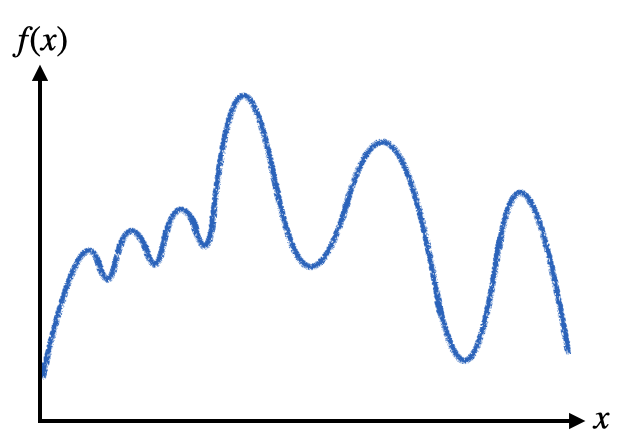
\includegraphics[width=.5\textwidth]{"Part 2 - Search-Based Optimization/Introduction/landscape.png"}
\caption{Example of objective landscape for an illustrative continuous optimization problem with a 1-dimensional design variable.}
\label{fig:landscape}
\end{figure}

\item \textit{Constraint(s)}  $g_i(\mathbf{x}) \leq 0$ and $h_j(\mathbf{x}) = 0$, where $i=\{1,2,\cdots,m\}$ and $j=\{1,2,\cdots,n\}$. These are the constraints that a candidate solution $\mathbf{x}$ needs satisfy in order to be a feasible solutions to the problem. When $m=0$ and $n=0$, the problem is called an unconstrained optimization problem. When $m>0$ or $n>0$, the problem is called a constrained optimization problem. 

The $g_i$ type of constraints are called \textit{inequality constraints}, whereas the $h_j$ type of constraints are called the \textit{equality constraints}. Problems may also involve constraints with inequalities of the type $\geq$ instead of $\leq$. However, it is possible to convert inequalities of the type $\geq$ to inequalities of the type $\leq$, reason why the canonical form above lists only $\leq$ without loss of generality.

Strict inequalities ($>$ or $<$) are typically not used in optimization problems, as they can lead to ill-posed problems. For instance, consider a problem where we wish to minimize $f(x) = x^2$, subject to $x>0$, where $x$ is a real value. Had the constraint been $x \geq 0$, the optimal solution would have been $x=0$. However, as the constraint is $x>0$, there is no minimizing value. In particular, we can always get $x$ values that are closer and closer and close to zero, without ever reaching a minimum. Alternatively, if $x$ was an integer value, this problem would not occur. However, in this case, it would be possible to convert the strict inequality $x>0$ into the inequality $x\geq 1$, meaning that the canonical form of the optimization problem does not need to have strict inequality constraints.

Some people also use terms such as \textit{hard constraints} and \textit{soft constraints}. When such terms are used, hard constraints refer to constraints that must be satisfied for the solution to be feasible, whereas soft constraints are constraints that we wish to satisfy, but that do not really lead to infeasible solutions when violated.
\end{itemize}

In order to formulate an optimization problem, all the components above must be specified. The more mathematical the problem formulation is, the less ambiguous it is likely to be. However, more mathematical formulations typically become more abstract, meaning that it may become more difficult to understand its underlying meaning in the context of the problem of interest. Therefore, it is advisable to provide a problem formulation that is the most formal (mathematical) possible, while also including an explanation of it using natural language. %Some examples of problem formulations are provided in the lecture slides.

%\section{Dealing with Constraints}
%
%Optimization algorithms from the artificial intelligence literature frequently don't include themselves strategies to deal with constraints. Instead, we need to design such strategies. There are many different ways to deal with constraints in optimization algorithms. Two examples of strategies are the following:
%
%\begin{itemize}
%\item Representation, initialisation and neighbourhood operators: this kind of strategy requires to design a representation, initialisation procedure and neighbourhood operators that do not allow any infeasible solution to ever be generated by the optimization algorithm. Its advantage is that it makes the optimization algorithms complete, i.e., guaranteed to find feasible solutions. Its disadvantage is that it is problem-dependent and thus not easy to design. Moreover, it may restrict the search space too much, which can sometimes hinder the search for optimal solutions. In the worse case scenario, such restrictions may eliminate the optimal solution from the reachable areas of the search space, meaning that the optimal solution cannot be found. 
%
%Some optimization algorithms are not based on neighbourhood operators, but other kinds of operators. In such cases, these other kinds of operators must also ensure that infeasible solutions are never generated.
%
%\item Objective function: it is possible to modify the objective function in order to penalise the objective values of infeasible solutions. Considering the general form of optimization problems shown in Section \ref{sec:formulation} with $k=1$, the objective function could be modified as shown below in order to deal with the constraints.
%
%\[
%\begin{tabular}{ll}
%minimize        & $f(\mathbf{x}) + Q(\mathbf{x})$\\
%subject to      & $g_i(\mathbf{x}) \leq 0$, \ \ \ \ \ $i=\{1,2,\cdots,m\}$ \\
%                & $h_j(\mathbf{x}) = 0$, \ \ \ \ \ $j=\{1,2,\cdots,n\}$ \\
%\end{tabular}
%\]
%
%\noindent where:
%
%\[ Q(\mathbf{x}) =
%  \begin{cases}
%    0       & \text{if } \mathbf{x} \text{ is feasible.}\\
%    P [g_a(\mathbf{x})^2 + g_b(\mathbf{x})^2 + \cdots + h_{a'}(\mathbf{x})^2 + h_{b'}(\mathbf{x})^2 + \cdots] & \text{otherwise}
%  \end{cases}
%\]
%
%\noindent where $P$ is a very large positive constant, and the indexes $a$, $b$, ..., $a'$, $b'$, ..., represent the indexes of the constraints that are violated. For example, consider a candidate solution $\mathbf{x}$ that violates only the constraints $g_2(\mathbf{x})$, $g_5(\mathbf{x})$ and $h_3(\mathbf{x})$. In this case, $Q(\mathbf{x}) = P [g_2(\mathbf{x})^2 + g_5(\mathbf{x})^2 + h_3(\mathbf{x})^2]$. The constant $P$ should ideally be large enough to make the objective value of infeasible solutions worse (larger) than the objective value of any feasible solution. The power of two used in the functions $g$ and $h$ ensures that the values of these functions will always be positive, such that the penalty will always increase (worsen) the objective value. % \footnote{The use of square can also help the optimization process depending on the optimization algorithm being adopted. This is because it causes the values of the objective function of infeasible solutions that violate a given constraint by different amounts to differ more from each other. For example, consider an infeasible solution $\mathbf{x}$ for which $g_a(\mathbf{x}) = 1$ and another infeasible solution $\mathbf{x}$ for which $g_a(\mathbf{x}) = 2$. The penalty applied to these }.
%
%The advantage of this strategy to deal with constraints is that it is very general. The same strategy could potentially be adopted for any optimization problem. However, as it enables infeasible solutions to be generated, the optimization algorithm would have to spend time searching for feasible solutions. For some problems where that are too many infeasible solutions, the algorithm may struggle to find feasible solutions based solely on the objective function, in which case the strategy based on representation, initialisation and neighbourhood operators may be more adequate. 
%
%An example of use of these two types of strategies to deal with constraints is provided in the lecture slides.
%
%
%\end{itemize}

\section{Search-Based Optimization Algorithms}
\label{sec:alg}

\textit{Optimization algorithms} are algorithms that attempt to find optimal solutions to optimization problems. \textit{Search-based optimization algorithms} are computational intelligence algorithms that conduct a search process in an attempt to find an optimal solution. They typically create one (or more) full initial candidate solutions to the problem, and then try to iteratively improve such candidate solution(s) to search for an optimal solution. When multiple candidate solutions are created and maintained at each iteration, the algorithm is typically called a \textit{population-based} algorithm, in contrast to algorithms that create and keep a \textit{single individual} candidate solution in each iteration. It is worth noting that these algorithms are different from search tree-based search algorithms, which attempt to systematically explore the search space to find actions that build a solution step-by-step over time instead of creating full candidate solutions from the beginning. 

For example, consider a routing problem where we wish to find a path to go from a given city A to city F. Consider also that cities B, C, D, E, G, H are also cities in the map. A search tree-based algorithm would start with city A, and then it may add city B to this path, and then add city C, and so on, until a full path between city A and city F is found. Such path is being constructed over time by systematically exploring the space of possible paths in the problem.

In contrast, a search-based optimization algorithm to solve a routing problem might start with an initial solution which consists of a vector of cities [A, B, C, G]. The algorithm would consider this to be a full \textit{candidate} solution to the problem, despite it being infeasible -- it does not reach the destination city F. The algorithm would then modify this candidate solution over time, possibly by replacing, adding or removing cities, in an attempt to find better candidates solutions to the problem. 

Search-based optimization algorithms typically do not maintain a data structure to store all the explored portion of the space of possible solutions to the problem, being usually more space-efficient than search tree-based algorithms. Several optimization algorithms from the computational intelligence literature are also more time efficient than the search tree-based algorithms, depending on the problem that is being solved. In addition, they usually do not require problem-specific heuristics\footnote{Heuristics are functions designed based on prior knowledge about a given problem that can be used to solve such problem more efficiently, despite possibly loosing, e.g., in optimality guarantees.} that are difficult to design, which is an advantage over tree-based search algorithms such as A*. As they are multi-purpose frameworks that can be used to solve a variety of problems, they are typically referred to as \textit{meta-heuristics}. In particular, by following such frameworks, it is possible to develop heuristics for a variety of different optimization problems.

%Optimization algorithms from the computational intelligence literature are frequently \textit{not guaranteed} to find optimal or feasible solutions, but will frequently be able to find good (or near optimal) solutions in a reasonable amount of time.



%\bibliographystyle{unsrt}
%\bibliography{bibliography}


\todo{Define heuristic and meta-heuristic}

\todo{Exploration and exploitation}

\todo{For ML, mention noise}